\section{Simulated Annealing}

\begin{frame}
\frametitle{Simulated Annealing}
    \begin{block}{Metropolis-Funktion}
        \begin{equation}
            p =
            \begin{cases}
                1 & \text{falls } e_{i+1} \ge e_i \\
                exp(- \frac{e_i - e_{i+1}}{t_i}) & \text{falls } e_{i+1} < e_i \notag
            \end{cases}
        \end{equation}
    \end{block}
    \begin{block}{Bestimmung der Nachbarn}
       \begin{equation}
           a_{i}^{'} =
           \begin{cases}
               a_i + (h_i - a_i) \cdot r_2 & \text{falls } r_1 > 0.5 \\
               a_i - (a_i - l_i) \cdot r_2 & \text{falls } r_1 \le 0.5 \notag
           \end{cases}
       \end{equation}
   \end{block}
\end{frame}

\subsection{Einstellbare Parameter}

\begin{frame}
\frametitle{Einstellbare Parameter}
    \begin{columns}
        \column[t]{.5\textwidth}
        \begin{itemize}
            \item maxsteps
            \item start\_temperature
            \item cooling\_schedule
            \item cooling\_schedule\_alpha
            \item neighbour\_count
        \end{itemize}
        \column[t]{.5\textwidth}
        \begin{block}{Abkühlung}
           Linear: \centerline{$ t_{i+1} = t_0 \cdot ( 1 - \frac{i}{i_{max}}) $} \\
           Exponentiell: \centerline{$ t_{i+1} = t_0 \cdot \alpha^i $} \\
        \end{block}
    \end{columns}
\end{frame}

\subsection{Ergebnisse}

\begin{frame}
\frametitle{Ergebnisse}
    \begin{figure}
        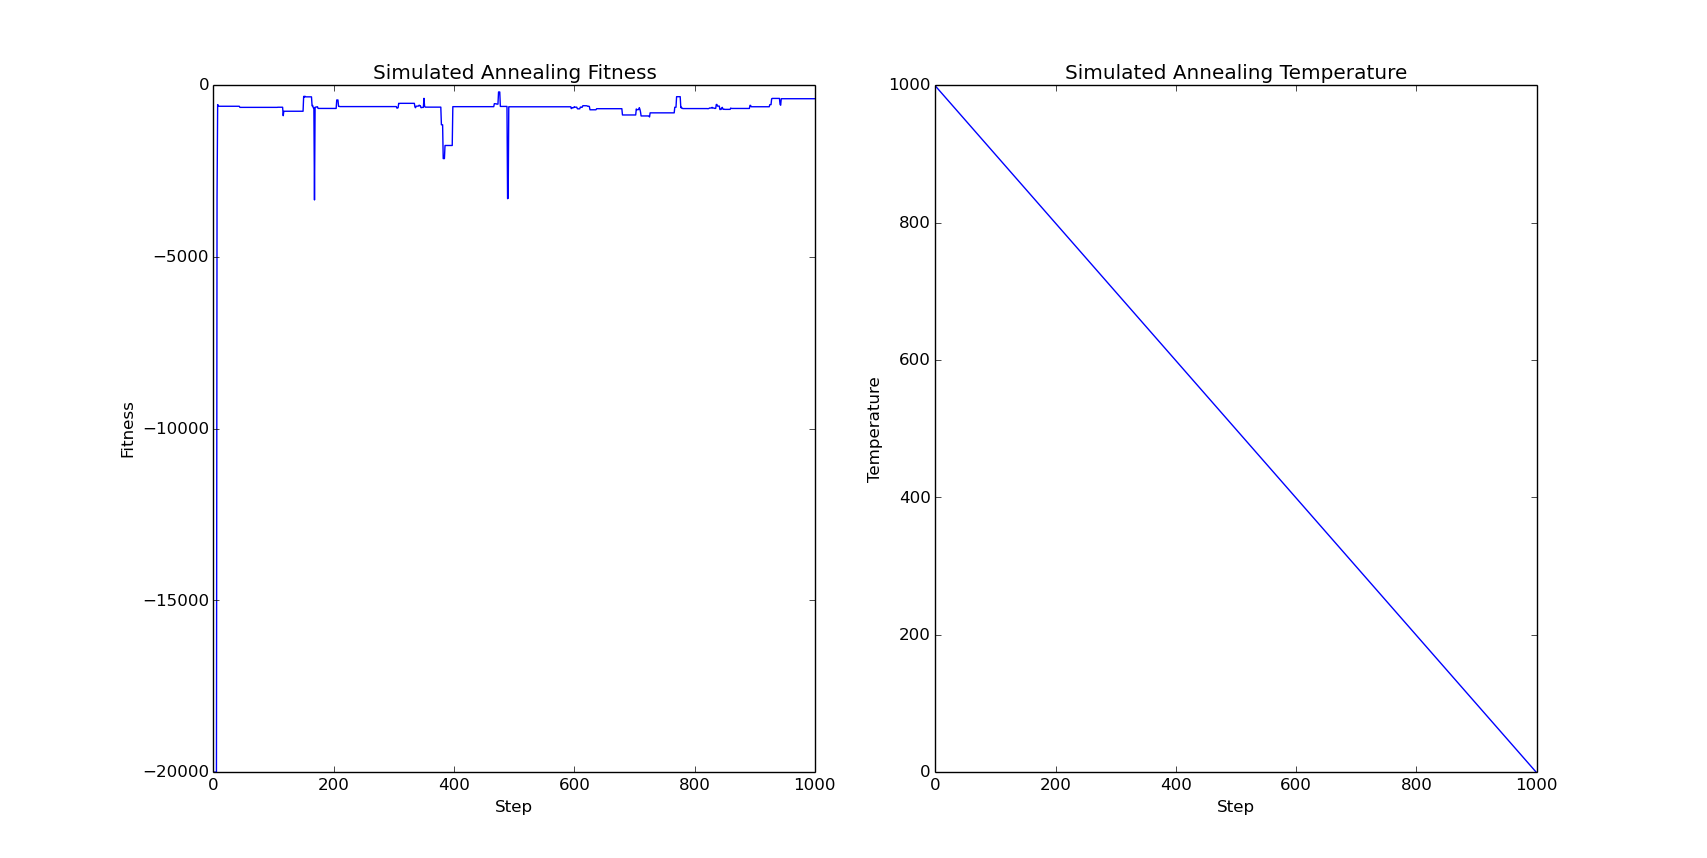
\includegraphics[width=\textwidth]{sa-gs/lin_ok.png}
        \caption{Lineare Abkühlung mit Starttemperatur 1000}
    \end{figure}
\end{frame}


\begin{frame}
\frametitle{Ergebnisse}
    \begin{figure}
        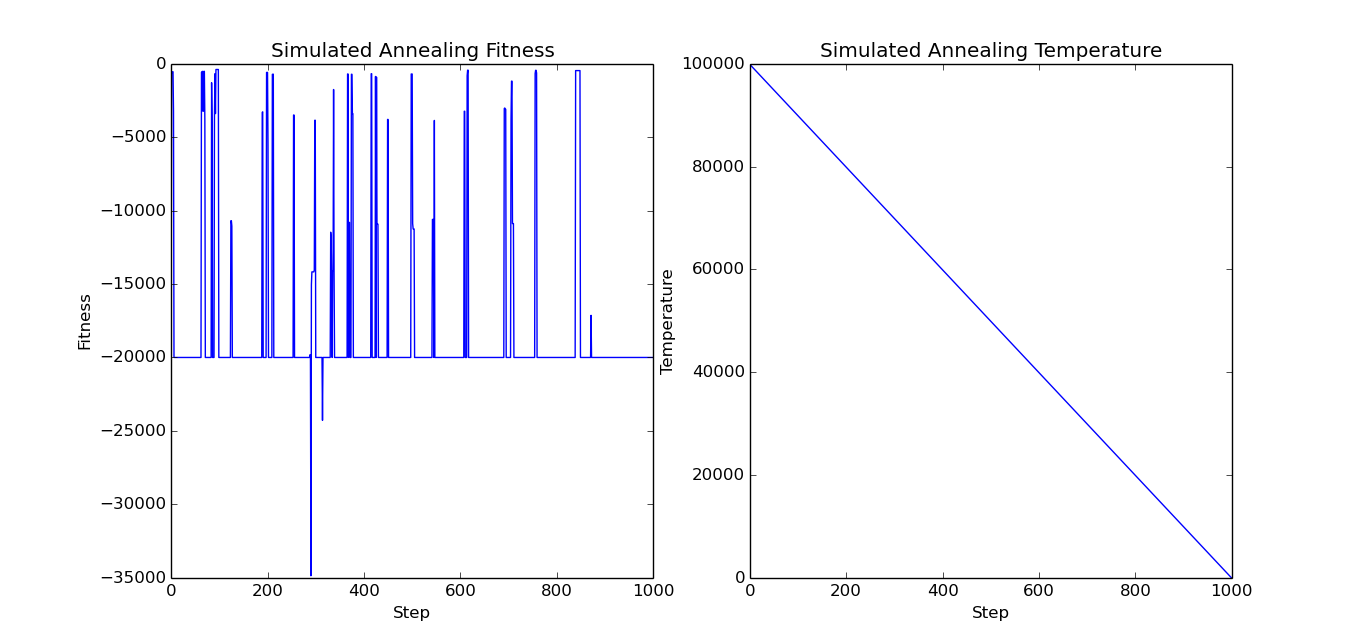
\includegraphics[width=\textwidth]{sa-gs/lin_doof.png}
        \caption{Lineare Abkühlung mit Starttemperatur 100000}
    \end{figure}
\end{frame}

\begin{frame}
\frametitle{Ergebnisse}
    \begin{figure}
        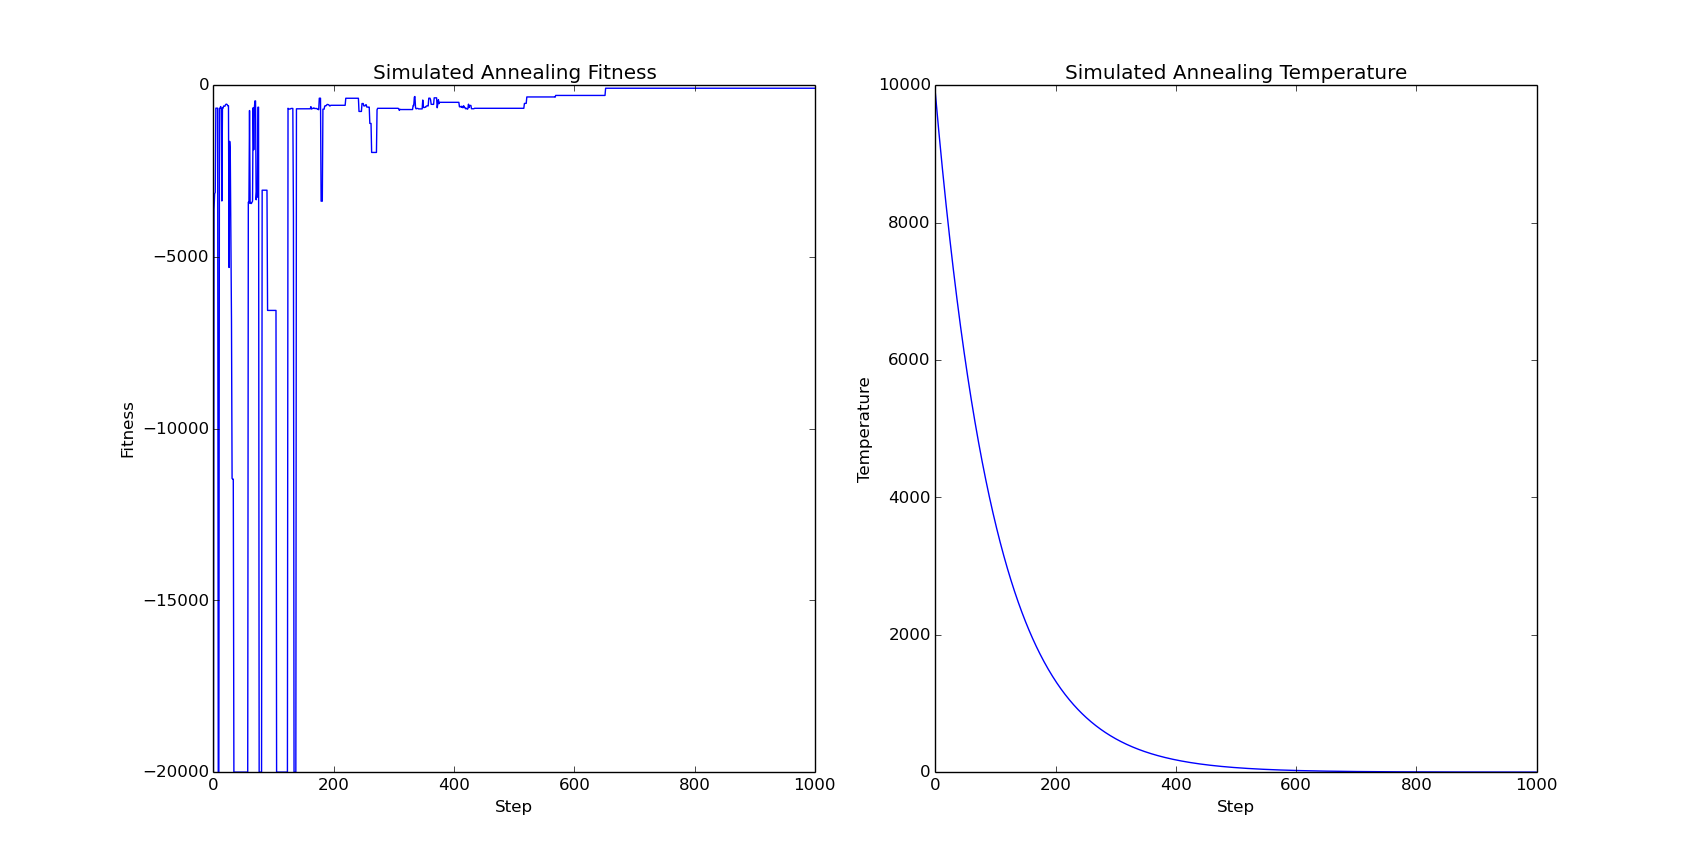
\includegraphics[width=\textwidth]{sa-gs/exp_gut.png}
        \caption{Exponentielle Abkühlung mit Starttemperatur 10000}
    \end{figure}
\end{frame}

%\begin{frame}
%\frametitle{Ergebnisse}
%    \center
%    \begin{figure}
%        \begin{tabular}{|ccc|}
%            \hline
%            Neuron & Linear & Exponentiell \\
%            \hline
%            RS & -20000 & -20000 \\
%            FS & -20000 & -20000 \\
%            IB & -20000 & -20000 \\
%            CH & -20000 & -20000 \\
%            \hline
%        \end{tabular}
%    \caption{Fitnesswerte nach 1000 Schritten}
%    \end{figure}
%\end{frame}

\subsection{Erweiterungen}

\begin{frame}
\frametitle{Erweiterungen}
    \begin{itemize}
        \item Übergeben eines Startchromosoms
        \item Erweiterung der Nachbarschaftssuche
            \begin{itemize}
                \item Mehrere Kanäle gleichzeitig verändern
                \item Konstante Schrittweite der Kanalwerte
            \end{itemize}
        \item Dynamische Abkühlung
    \end{itemize}
\end{frame}
